\documentclass[11pt,a4paper]{article}
\usepackage[T1]{fontenc}
\usepackage[utf8]{inputenc}
\usepackage[polish]{babel}
\usepackage{lmodern}
\usepackage[a4paper,margin=2.5cm]{geometry}
\usepackage{graphicx}
\usepackage{booktabs}
\usepackage{amsmath}
\usepackage{xcolor}
\usepackage{listings}
\usepackage{caption}
\usepackage[colorlinks=true,linkcolor=blue!50!black,citecolor=blue!50!black,urlcolor=blue!50!black]{hyperref}
\usepackage{float}

\captionsetup{font=small,labelfont=bf}
\captionsetup[table]{position=above}
\captionsetup[figure]{position=below}

\definecolor{kwcol}{RGB}{40,60,130}
\definecolor{cmcol}{RGB}{90,120,90}
\definecolor{nrcol}{RGB}{130,130,130}
\definecolor{bgcol}{RGB}{248,248,248}

\lstdefinestyle{cpp}{
  language=C++,
  basicstyle=\ttfamily\scriptsize,
  keywordstyle=\color{kwcol},
  commentstyle=\color{cmcol}\itshape,
  stringstyle=\color{brown!70!black},
  numbers=left,
  numberstyle=\tiny\color{nrcol},
  numbersep=6pt,
  backgroundcolor=\color{bgcol},
  frame=single,
  rulecolor=\color{nrcol!50},
  breaklines=true,
  showstringspaces=false,
  tabsize=4,
  columns=fullflexible,
  keepspaces=true,
  literate={ą}{{\k{a}}}1 {ć}{{\'c}}1 {ę}{{\k{e}}}1 {ł}{{\l}}1 {ń}{{\'n}}1
           {ó}{{\'o}}1 {ś}{{\'s}}1 {ź}{{\'z}}1 {ż}{{\.z}}1
           {Ą}{{\k{A}}}1 {Ć}{{\'C}}1 {Ę}{{\k{E}}}1 {Ł}{{\L}}1 {Ń}{{\'N}}1
           {Ó}{{\'O}}1 {Ś}{{\'S}}1 {Ź}{{\'Z}}1 {Ż}{{\.Z}}1
           {×}{{$\times$}}1 {—}{{---}}1 {→}{{$\to$}}1,
}
\lstdefinestyle{plain}{style=cpp,language={},numbers=none}
\lstset{style=cpp}

\title{Laboratorium 3: równoległa konwolucja 2D w OpenMP}
\author{Jakub Balicki}
\date{2026-11}

\begin{document}
\maketitle
\vspace{-1em}

\section{Zadanie i implementacja}
Program liczy konwolucję 2D macierzy \texttt{float} ($N\times N$) z jądrem $K\times K$ ($K$ nieparzyste), z zerowym dopełnieniem poza obrazem:
\begin{equation}
  w_{ij}=\sum_{m=0}^{K-1}\sum_{n=0}^{K-1} M\!\left[i+m-\lfloor K/2\rfloor\right]\!\left[j+n-\lfloor K/2\rfloor\right]\,J[m][n].
\end{equation}
Dane są losowe z $[-1,1]$ (\texttt{mt19937}), jądro jest normalizowane sumą wartości bezwzględnych. Trzy warianty równoległe mają to samo ciało pętli i różnią się tylko dyrektywą:
\begin{lstlisting}
// 1) podzial wierszy na bloki po ~H/p
#pragma omp parallel for num_threads(num_threads) schedule(static)
// 2) petle i oraz j sklejone w jedna przestrzen H*W iteracji
#pragma omp parallel for collapse(2) num_threads(num_threads) schedule(static)
// 3) wiersze rozdawane dynamicznie, po 64 naraz
#pragma omp parallel for num_threads(num_threads) schedule(dynamic, 64)
\end{lstlisting}

Pomiary: AMD Ryzen 7 5700X (8 rdzeni, 16 wątków sprzętowych, L3 32\,MiB), Linux, \texttt{g++ -O2 -fopenmp}. Konfiguracje: $512^2$ z jądrem $3\times3$, $2048^2$ z $7\times7$ i $4096^2$ z $15\times15$, każda dla 1, 4 i 8 wątków. Czas to pojedynczy pomiar \texttt{omp\_get\_wtime()} samej konwolucji, a baza sekwencyjna jest mierzona w tym samym uruchomieniu. Wszystkie 27 porównań z wynikiem sekwencyjnym dało zgodność do $10^{-4}$.

\section{Wyniki}
\begin{table}[H]
\centering
\caption{Przyspieszenie $S=T_{\mathrm{seq}}/T_{\mathrm{par}}$ względem wersji sekwencyjnej z tego samego uruchomienia.}\label{tab:speedup}
\begin{tabular}{llrrr}
\toprule
Obraz, jądro & Wątki & \texttt{parallel for} & \texttt{collapse(2)} & \texttt{dynamic,\,64} \\
\midrule
$512\times512$, $3\times3$     & 1 & 1,13 & 1,05 & 1,36 \\
                               & 4 & 2,58 & 2,81 & 2,42 \\
                               & 8 & 3,67 & 4,19 & 4,69 \\
\midrule
$2048\times2048$, $7\times7$   & 1 & 1,05 & 1,15 & 1,03 \\
                               & 4 & 3,46 & 4,21 & 3,34 \\
                               & 8 & 4,38 & 4,89 & 5,06 \\
\midrule
$4096\times4096$, $15\times15$ & 1 & 1,05 & 1,07 & 1,07 \\
                               & 4 & 3,91 & 4,08 & 4,09 \\
                               & 8 & 5,06 & 5,04 & 5,76 \\
\bottomrule
\end{tabular}
\end{table}

\begin{table}[H]
\centering
\caption{Czasy wykonania [s] dla 8 wątków (jedno uruchomienie, zaokrąglenie do 1\,ms przez program).}\label{tab:czasy}
\begin{tabular}{lrrrr}
\toprule
Obraz, jądro & Seq & \texttt{parallel for} & \texttt{collapse(2)} & \texttt{dynamic,\,64} \\
\midrule
$2048\times2048$, $7\times7$   & 0,151 & 0,034 & 0,031 & 0,030 \\
$4096\times4096$, $15\times15$ & 2,639 & 0,522 & 0,523 & 0,458 \\
\bottomrule
\end{tabular}
\end{table}

\begin{figure}[H]
\centering
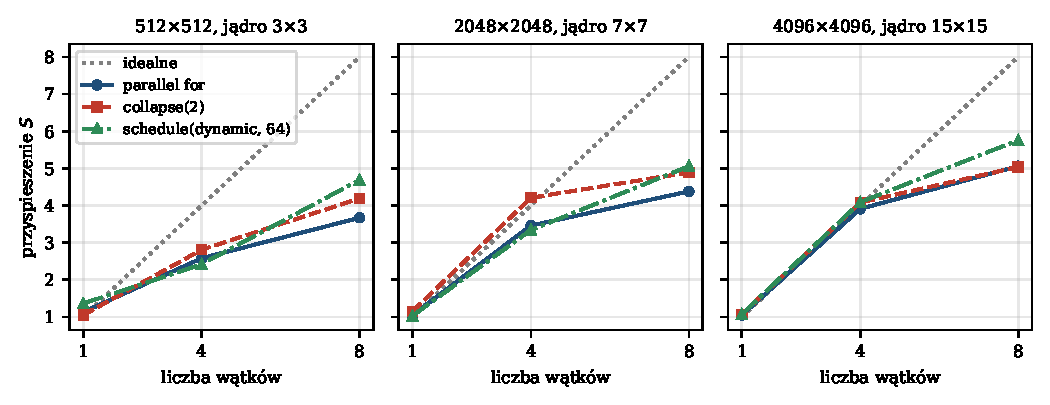
\includegraphics[width=0.85\textwidth]{fig_speedup.pdf}
\caption{Przyspieszenie względem liczby wątków; linia kropkowana to przyspieszenie idealne. Po jednym uruchomieniu na punkt.}\label{fig:speedup}
\end{figure}

\begin{figure}[H]
\centering
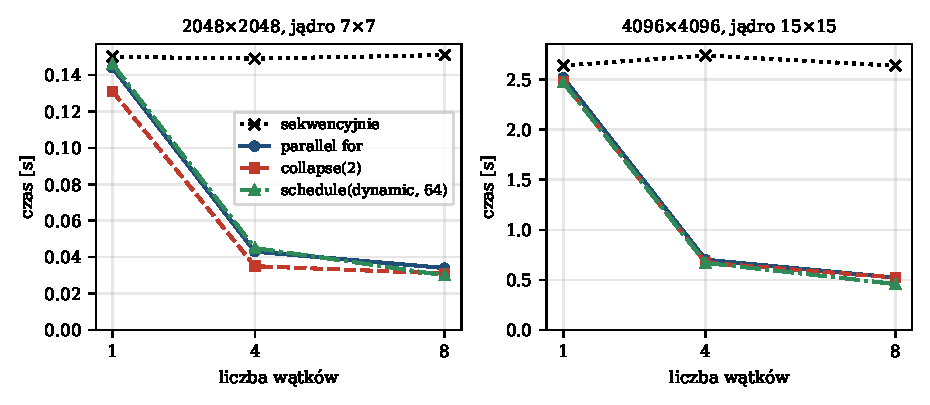
\includegraphics[width=0.8\textwidth]{fig_czas.pdf}
\caption{Czas konwolucji względem liczby wątków dla dwóch większych konfiguracji.}\label{fig:czas}
\end{figure}

\section{Wnioski}
\begin{itemize}
\item Przy 4 wątkach przyspieszenie wynosi 2,4--4,2 (ok.\ 4 dla dużych danych), a przy 8 wątkach 3,7--5,8. Dla dużych danych skalowanie przy 4 wątkach jest niemal liniowe, a przy 8 wątkach sprawność spada do 0,55--0,72.
\item Dla małego obrazu ($512^2$, czasy 2--3\,ms) przyspieszenie jest najniższe, bo koszt uruchomienia wątków i bariery jest porównywalny z obliczeniem.
\item \texttt{parallel for} i \texttt{collapse(2)} dają ten sam podział pracy i zbliżone czasy; różnice mieszczą się w szumie pomiaru.
\item \texttt{dynamic,\,64} wypadł najlepiej przy 8 wątkach (5,76 dla $4096^2$, ok.\ 12\% szybciej od wariantów statycznych).
\item Wartości powyżej 4 przy 4 wątkach wynikają z tego, że wersja sekwencyjna jest mierzona jako pierwsza i bywa wolniejsza od równoległej na jednym wątku.
\end{itemize}

\end{document}
